%=======================02-713 LaTeX template, following the 15-210 template==================
%
% You don't need to use LaTeX or this template, but you must turn your homework in as
% a typeset PDF somehow.
%
% How to use:
%    1. Update your information in section "A" below
%    2. Write your answers in section "B" below. Precede answers for all 
%       parts of a question with the command "\question{n}{desc}" where n is
%       the question number and "desc" is a short, one-line description of 
%       the problem. There is no need to restate the problem.
%    3. If a question has multiple parts, precede the answer to part x with the
%       command "\part{x}".
%    4. If a problem asks you to design an algorithm, use the commands
%       \algorithm, \correctness, \runtime to precede your discussion of the 
%       description of the algorithm, its correctness, and its running time, respectively.
%    5. You can include graphics by using the command \includegraphics{FILENAME}
%
\documentclass[11pt]{article}
\usepackage{amsmath,amssymb,amsthm}
\usepackage{graphicx}
\usepackage[margin=1in]{geometry}
\usepackage{fancyhdr}
\setlength{\parindent}{0pt}
\setlength{\parskip}{5pt plus 1pt}
\setlength{\headheight}{13.6pt}
\newcommand\question[2]{\vspace{.25in}\hrule\textbf{#1: #2}\vspace{.5em}\hrule\vspace{.10in}}
\renewcommand\part[1]{\vspace{.10in}\textbf{(#1)}\par}
\newcommand\algorithm{\vspace{.10in}\textbf{Algorithm: }}
\newcommand\correctness{\vspace{.10in}\textbf{Correctness: }}
\newcommand\runtime{\vspace{.10in}\textbf{Running time: }}
\pagestyle{fancyplain}
\lhead{\textbf{\NAME}}
\chead{\textbf{{\COURSE} HW\HWNUM}}
\rhead{\today}
\begin{document}\raggedright
%Section A==============Change the values below to match your information==================
\newcommand\NAME{Eric Altenburg}  % your name
\newcommand\COURSE{MA-331}
\newcommand\HWNUM{6}              % the homework number
%Section B==============Put your answers to the questions below here=======================

% no need to restate the problem --- the graders know which problem is which,
% but replacing "The First Problem" with a short phrase will help you remember
% which problem this is when you read over your homeworks to study.

\textit{Pledge: I pledge my honor that I have abided by the Stevens Honor System.} -Eric Altenburg

\question{12.31}{Page 682-683}
	\part{a}
		\begin{tabular}{|c|c|c|c|}
			\hline
			Groups & Sample Size & Mean & Std. Deviation\\
			\hline
			Control & 35 & -1.0086 & 11.5007\\
			\hline
			Individual & 35 & -3.7086 & 9.0784\\
			\hline
			Group & 34 & -10.7853 & 11.1392\\
			\hline
		\end{tabular}
	
	\part{b}
		Yes it is reasonable to pool the variances because the following holds true:\par
		$2 * 9.0784 = 18.1568 > 11.5007$\par
	\part{c}
		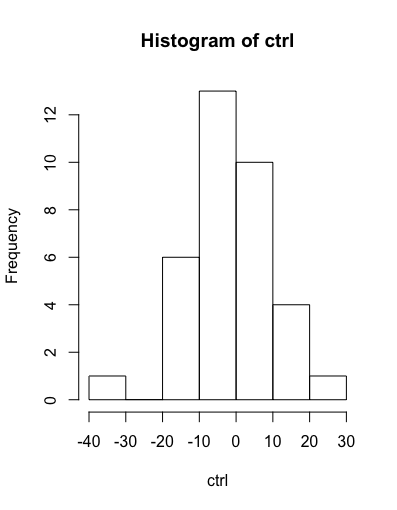
\includegraphics[scale=0.38]{images/ctrlHist.png}
		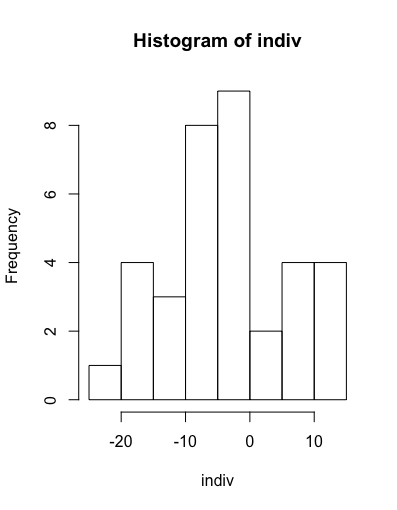
\includegraphics[scale=0.38]{images/indivHist.png}
		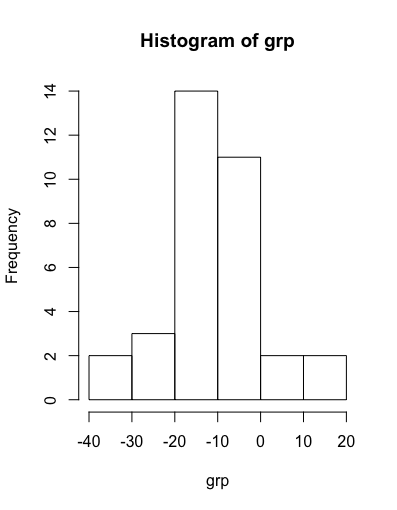
\includegraphics[scale=0.38]{images/grpHist.png}\par
		
		From these histograms, one can draw the conclusion that the sample means are approximately normal because although the control seems to be more of a symmetric distribution and the individual is right-skewed, the sample sizes are around 34, therefore, if the samples do not exactly represent a normal distribution, it is acceptable.\par
	

\question{12.32}{Page 683}
	\part{a}
		We define $H_{0}: \mu_{1} = \mu_{2} = \mu_{3}$ versus $H_{a}:$ they are not all equal.\par
		\begin{align*}
			\overline{X}_{.,.} &= \frac{(35(-1.0086) + 35(-3.7086) + 34(-10.7853)}{104}\\
			&= -5.1135\\
			SSB &= \Sigma^{3}_{i=1} n_{i}(\overline{X}_{i,.}-\overline{X}_{.,.})^{2}\\
			&= 1752.5945\\
			SSE &= \Sigma^{3}_{i=1}(n_{i}-1)S^{2}_{i}\\
			&= 11393.9358\\
			f &= \frac{\frac{SSB}{k-1}}{\frac{SSE}{n-k}}\\
			&= 7.7678\\
			df &= 2\\
			P(F>7.7678) &= 1-pf(7.7678, 2, 101) = 0.0007278958 << 0.05 = \alpha\\
		\end{align*}\par
		\begin{tabular}{|c|c|c|c|c|c|}
			\hline
			Source & df & SS & MS & F statistic & p-value\\
			\hline
			Group & 2 & 1752.5945 & 876.2973 & 7.7678 & 0.0007278958\\
			\hline
			Error & 101 & 11393.9358 & 112.8112 & &\\
			\hline
			Total & 103 & 13146.5303 &&&\\
			\hline
		\end{tabular}\par
		Since the p-value is less than the significance level of 0.05, we reject $H_{0}$ which states that $\mu_{1}, \mu_{2}, \mu_{3}$ are not all equal.\par
		
	
	\part{b}
		From Professor Li's announcement via Canvas:\par
		\begin{quotation}
		regarding 12.32 b
		
		Hi, there,

		Please forget the residual analysis in Question 12.32 (b), which is not considered in our slides.

		Regards,
		
		Xiaohu Li
		\end{quotation}\par
	
	\part{c}
		\begin{align*}
			T_{i,j} &= \frac{ \overline{X}_{i,.} - \overline{X}_{j,.}}{ \sqrt{S^{2}_{p}(\frac{1}{n_{i}} + \frac{1}{n_{j}})} }\\
			S^{2}_{p} &= \frac{SSE}{n-k}=112.8019\\
			Individual-Control &= |-1.0634|\\
			Individual-Group &= |-2.7671|\\
			Control-Group &= |-3.8228|\\
		\end{align*}\par
		
		\begin{align*}
			P(|T_{i,j}| > |t_{i,j}|) &= 2[1-pt(|t_{i,j}|, n-k)] < \alpha \\
			n-k &= 104-3=101\\
			Individual-Control &= 0.2901365\\
			Individual-Group &= 0.006727696\\
			Control-Group &= 0.0002283676\\
		\end{align*}\par
		
		Based on the LSD method:\par
		Individual-Control, 0.2901365 $>$ 0.05, therefore, we fail to reject $H_{0}$ saying that $\mu_{individual}=\mu_{control}$.\par
		Individual-Group, 0.0067276965 $<$ 0.05, therefore, we reject $H_{0}$ saying that $\mu_{individual} \ne \mu_{group}$.\par
		Control-Group, 0.0002283676 $<$ 0.05, therefore, we reject $H_{0}$ saying that $\mu_{control} \ne \mu_{group}$.\par
	\part{d}
		Based on the ANOVA test in part (a), it is clear that the means are different among each group. Using the LSD method from part (c) shows that the outlier causing the means to be different in part (a) was the group-incentive program as individual and control both had equal means, but in both of the group-incentive pairings, it rejected the $H_{0}$ stating that the two means are not equal.\par
	

\question{12.33}{Page 683}
	\part{a}
		The new means and standard deviations for each of the groups would still remain the same, however, they would just be divided by 2.2:\par
		\begin{tabular}{|c|c|c|c|}
			\hline
			Groups & Sample Size & Mean & Std. Deviation\\
			\hline
			Control & 35 & -0.4585 & 5.2276\\
			\hline
			Individual & 35 & -1.6857 & 4.1265\\
			\hline
			Group & 34 & -4.9024 & 5.0632\\
			\hline
		\end{tabular}\par
	
	\part{b}
		\begin{tabular}{|c|c|c|c|c|c|}
			\hline
			Source & df & SS & MS & F statistic & p-value\\
			\hline
			Group & 2 & 362.1000 & 181.0500 & 7.7678 & 0.0007278958\\
			\hline
			Error & 101 & 2354.0851 & 23.3077 & &\\
			\hline
			Total & 103 & 2716.1851 &&&\\
			\hline
		\end{tabular}\par
		Based on these findings, dividing by 2.2 did not change the normality of the data, therefore, the values are the same as the previous problem and so are the findings in regards to the hypotheses. \par


\question{12.41}{Page 685}
		$\mu_{1}$ = Blue Eyes\par
		$\mu_{2}$ = Brown Eyes\par
		$\mu_{3}$ = Down Eyes\par
		$\mu_{4}$ = Green Eyes\par
	\part{a}
		Compare the average of brown eyes to the average of another color eye:\par
		$\psi_{1}=\mu_{2} - \frac{(\mu_{1} + \mu_{4})}{2}$\par
	
	\part{b}
		Compare down eyes to the rest of the eyes:\par
		$\psi_{2} = \frac{(\mu_{1} + \mu_{2} + \mu_{4})}{3}-\mu_{3}$


\question{12.42}{Page 685}
	\part{a}
		$\Psi_{1}, H_{0}: \Psi_{1} = 0$\par
		$\Psi_{1}, H_{a}: \Psi_{1} \ne 0$\par
		$\Psi_{2}, H_{0}: \Psi_{2} = 0$\par
		$\Psi_{2}, H_{a}: \Psi_{2} \ne 0$\par
	
	\part{b}
		$c_{1} = 3.72 - \frac{7.05}{2} = 0.195$\par
		$c_{2} = \frac{3.19 + 3.72 + 3.86}{3} - 3.11= 0.48$\par	
	
	\part{c}
		\begin{align*}
			S_{p} &= \sqrt{ \frac{ (67-1)(1.65)(2) + ... }{ (67-1) + ... } } = 1.68\\
			SE_{c_{1}} &= 1.68 * \sqrt{\frac{1}{37}+ \frac{\frac{-1}{4}}{67} + \frac{\frac{-1}{4}}{77}} = 0.3098\\
			SE_{c_{2}} &= 1.68 * \sqrt{  \frac{\frac{1}{9}}{67} + \frac{\frac{1}{9}}{37} + \frac{\frac{1}{9}}{77} + \frac{1}{41}} = 0.2933\\
		\end{align*}\par
	
	\part{d}
		\begin{align*}
			t_{1} &= \frac{c_{1}}{SE_{c_{1}}} = \frac{0.195}{0.3098} = 0.631\\
			df &= n-k =218\\
			P(|T| > |t|) &= 2[1-pt(|t|, n-k)] < \alpha \\
			p-value &= 0.5228446 > 0.05 = \alpha\\
		\end{align*}\par
		Based on this p-value, since it is not less than the significance level of 0.05, we fail to reject $H_{0}$.\par
		\begin{align*}
			t_{2} &= \frac{0.48}{0.2933} = 1.64\\
			df &= 218\\
			P(|T| > |t|) &= 2[1-pt(|t|, n-k)] < \alpha \\
			p-value &= 0.1024473 > 0.5 = \alpha\\
		\end{align*}\par
		Based on this p-value, since it is not less than the significance level of 0.05, we fail to reject $H_{0}$.\par
	
	\part{e}
		For $c_{1}$:\par
		$0.195 \pm 1.96 * 0.309 = 0.195 \pm 0.6564 = (-0.41064, 0.80064)$\par
		For $c_{2}$:\par
		$0.48 \pm 1.96 * 0.293 = 0.48 \pm 0.57428 = (-0.09428, 1.05428)$\par


\end{document}